\documentclass[a4paper,12pt,final,oneside,openright]{article}
\usepackage{report}

\newcommand{\reporttitle}{Search Engines and Information Retrieval Systems}
\newcommand{\enseignants}{
Johan Boye\\
Carl Eriksson\\
Jussi Karlg\\
Hedvig Kjellström\\
Sahar Asadi\\
Roelof Pieters}

\newcommand{\reportauthor}{
Benjamin Coors\\
Rémi Domingues\\
Håkan Eriksson\\
Paul Griffin\\
Akash Kumar Dhaka}
% \newcommand{\hexanome}{H4211}
\newcommand{\reportsubject}{}
\newcommand{\stagetopic}{Virality Prediction}
\newcommand{\dateperiod}{April $15^{th}$ - May $22^{nd}$}
\newcommand{\HRule}{\rule{\linewidth}{0.5mm}}
\setlength{\parskip}{1ex} % Espace entre les paragraphes

\hypersetup{
    pdftitle={\reporttitle},%
    pdfauthor={\reportauthor},%
    pdfsubject={\reportsubject},%
    pdfkeywords={}
}

\title{\reporttitle}
\author{\reportauthor}

\setlongtables
\usepackage[font=small,skip=0pt]{caption}
\usepackage{algorithm}
\usepackage{algpseudocode}
\usepackage{listings}


%\setcounter{tocdepth}{4}
\begin{document}
    \renewcommand{\chaptername}{} %\renewcommand{\thechapter}{}
    \renewcommand{\contentsname}{Contents}

    \pagestyle{empty}
    \pagenumbering{arabic}
    % Inspiré de http://en.wikibooks.org/wiki/LaTeX/Title_Creation
\begin{center}
	\begin{minipage}[t]{0.48\textwidth}
	  \begin{flushleft}
	    
\includegraphics [width=30mm]{img/logo_kth.jpg} \\[0.1cm]
		Kungliga Tekniska Högskolan\\
		Valhallavägen 79\\
		100 44 Stockholm
	  \end{flushleft}
	\end{minipage}
	\begin{minipage}[t]{0.48\textwidth}
	  \begin{flushright}
	  \end{flushright}
	\end{minipage} \\[0.8cm]

	\textsc{\Large \reportsubject}\\[0.3cm]
	\HRule \\[0.4cm]
	{\Huge \bfseries \reporttitle}\\[0.3cm]
	{\LARGE \bfseries «~\stagetopic~»}\\[0.3cm]
	{\Large \dateperiod}\\[0.4cm]
	\HRule \\[1.5cm]

	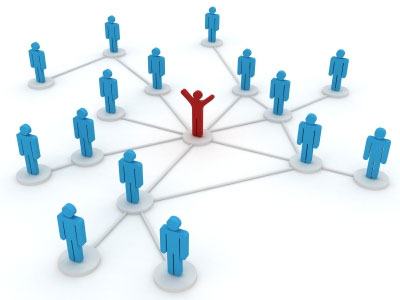
\includegraphics [width=0.4\linewidth]{img/icon.jpg} \\[1.5cm]
	\begin{minipage}[t]{0.5\textwidth}
	  \begin{flushleft} \large
	    \emph{Authors}\\
	    \reportauthor
	  \end{flushleft}
	\end{minipage}
	\begin{minipage}[t]{0.4\textwidth}
	  \begin{flushright} \large
	    \emph{Teachers and supervisors} \\
	    \enseignants
	  \end{flushright}
	\end{minipage}

	\vfill
	\footnotesize{Scholar year 2014-2015}
\end{center}
    \pagebreak
    \sloppy          % Justification moins stricte : des mots ne dépasseront pas des paragraphes

%     %\frontmatter
%     \thispagestyle{empty}
%     \tableofcontents
%     \addtocontents{toc}{\protect\thispagestyle{empty}}
%     \pagebreak

    %\mainmatter
    \pagestyle{headings}
    %\renewcommand{\chaptermark}[1]{\markboth{\MakeUppercase{\chaptername\ \thechapter.\ #1}}{}}
    %\renewcommand{\sectionmark}[1]{\markright{\thesection{} #1}}

	\setcounter{page}{1} % Ignore cover and toc
    \begin{abstract}
\noindent The social media platform Twitter is a rich source of data, useful for a number of applications. For example, in marketing it can be useful to analyze the Twitter flow to direct and focus campaigns more effectively. In this report, we gather data from Twitter and run machine learning algorithms to predict the virality of tweets. This work presents a novel approach of combining the virality prediction of individual tweets with concepts from information retrieval to implement a system to predict the virality of hashtags on Twitter. Our results show some promise of accurately predicting virality, but further development and research will be needed to increase the reliability and accuracy of the application.
\end{abstract}

\section{Introduction}
\noindent Twitter is a a popular social network platform where users can send and read messages (or ``tweets'').
A tweet is characterized by having a maximum length of $140$ characters, containing regular text as well as special markers.
The markers are the hashtag sign (``\#'') and the at sign (``@''). These can be used to tag tweets by topic or to reply to other specific users respectively. 
Twitter has at the time of this report hundreds of million users, and an ever greater amount of tweets are sent every day.
The amount of data that can be gathered from this social platform is thus very large and complex, but valuable nonetheless.

One such form of data is that of popular, or viral, tweets and topics.
For the purposes of this report, we will use tweets to refer to both actual tweets and the topics they pertain.
Certain tweets are often retweeted by large amounts of people, becoming viral as even more people discover and share them with each other.
These popular tweets change and fluctuate constantly on Twitter, seemingly in an unpredictable fashion.
Determining beforehand if a tweet is likely to become viral is interesting in many ways.
For example, analyzing current trends and opinions is of vital importance to maximize the effectiveness of marketing and creating buzz around products.
In this report we will therefore examine if it is possible to determine if a topic can become viral by examining its contents and comparing it to historical data.


\section{Related work}
\noindent Asur and Huberman attempted in 2010 to estimate the box office revenues for movies based on the rate of tweets about a given movie. 
They concluded that a relatively simple model can be useful and even outperform other predictors\cite{asur10}, showing that it is possible to use data found in Twitter to find indications and make predictions.
The task is finding the elements that will be of most use for the model, in our case what elements of a topic or tweet makes them more likely to spread.
This question has been the subject of quite a few studies, often to ascertain the key aspects that seem to govern if a Twitter topic becomes viral or not.

One aspect that has been deemed important is that of community structures and how a topic spreads through its first few occurences.
Weng et al. proposed an indicator of how likely a topic or tweet is to become viral is by looking at its initial spread in different communities \cite{weng14}. 
They showed that if a tweet gets ``trapped'' within one or a few communities, they are less likely to spread very far beyond these.
By judging if a given tweet or topic has been found among several divergent communities, they can more easily determine if it is a universally relevant or ``hot'' topic that will thus be more likely to spread.
This method does however recquire additional data on the composition of different communities and how their users overlap.

Another approach to determining if a tweet is likely to go viral is by analyzing and modelling the contents of the tweets.
There is a wealth of information in this area of research, as there are many potential aspects to investigate.
Roja Bandari et al. studied news articles that were shared on Twitter and found that the source of the article, as well as what entities the article contained, played an important role in predicting virality \cite{bandari12}.
Tweets containing articles from esteemed or popular sources that write about well-known organizations, people or events indicated a higher likelihood of being retweeted.
Tangentally, users with a high amount of followers are also likely to be retweeted. 
Suh et al. found a strong correlation between the followers of a user and the likelihood of tweets going viral. Furthermore, they found that the use of hashtags and links also increase the likelihood of a tweet going viral \cite{suh10}.
However, they could not determine why certain popular hashtags produced many retweets while others did not.

Analyzing the sentiments of tweets has also been a topic of many studies, but appears difficult to reliably use to predict virality.
Hansen et al. suggested that news with negative sentiments were more likely to be retweeted than positive, while the reverse applied in generic tweet settings \cite{hansen11}.
Another article, by Berger and Milkman, points to the complexity of determining sentiment through the Twitter medium \cite{berger12}.
Their results suggests, somewhat contrary to Hansen et al., that positive news seem to be more likely to be shared.
Both studies indicates that sentiment has an impact on the virality of a tweet, but that measuring this property can be problematic.

Quantifying the sentiments is limited by the format of Twitter.
Sarcasm, humor and intent can often be elusive in the short and mostly textual messages of Twitter, and are thus not easily classified with regards to sentiment.
To accurately utilize sentiment analysis one would require resources beyond the scope of this report.






\section{Methodology}

% TODO - THis is just a rough draft of the methodlogy, feel free to edit it and add accordingly. 

For our implementation we decided to focus on the approach of predicting the virality of a tweet from its content and further important attributes of a tweet relative to others, which make it more popular. As the problem of virality prediction is very wide, we restricted the scope of the problem by focusing on the virality of hashtags by predicting the virality of the tweets containing a particular hashtag. We decided to define the virality of a tweet in terms of the number of retweets it obtained. As features for our predictor we chose some features related to the author of the tweet, such as the author's number of followers, friends, appearances on lists, statuses and favourites as well as the age of the account in days. Further, we included features related to the content of the tweet itself: the number of hashtags, media, user mentions, and URLs contained as well as the length of the tweet. 

\begin{figure}[H]
\centering
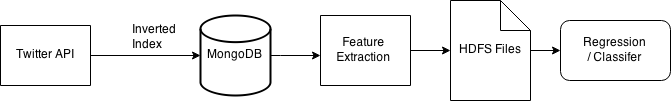
\includegraphics[width=0.7\linewidth]{img/pipeline.png}
\caption{Pipeline of our work}
\label{fig:pipeline}
\end{figure}



\subsection{Data retrieval}
Figure \ref{fig:pipeline} shows the pipeline of our data retrieval system. The first component is a crawler which aims at retrieving random English tweets using the Twitter streaming API, which gives developers access to Twitter’s global stream of tweet data. To receive a representative subset of tweets, the streaming API is queried for a list of English stop words, which are commonly contained in tweets.

Each tweet is returned as a JSON document and stored in a MongoDB instance. Further, each tweet is analyzed for hashtags. Based on the hashtags contained, an inverted index is created which contains the IDs of all tweets containing a particular hashtag. Three days after the data acquisition, the number of retweets of each tweet in the database is updated by performing an additional call to the Twitter API for each tweet. This time frame between the data retrieval and the retweet count update determines the scope of our predictions, i.e. the virality predictions made by our model will be valid for this specific time interval.

Once we have our raw data, the data needs to be cleaned before extracting features from it. Outliers with a very high retweet count and tweets which do not contain any hashtag are removed. Counters lower than 0 are set to 0 and tweets longer than 140 characters are set to 140. The selected features are mostly from metadata, which means that our current implementation does not analyse the text of the tweet to predict its virality. Such an approach would for example include sentiment analysis. The raw data stored in the database is not altered during this process, as we store the extracted features and the number of retweets in a HDF5 file.

\subsection{Data analysis}
\label{sec:analyis}
The following plots show the correlation between each feature (X-axis) and the number of retweets (Y-axis).

\begin{figure}[H]
\minipage[t]{0.25\textwidth}
    \centering
    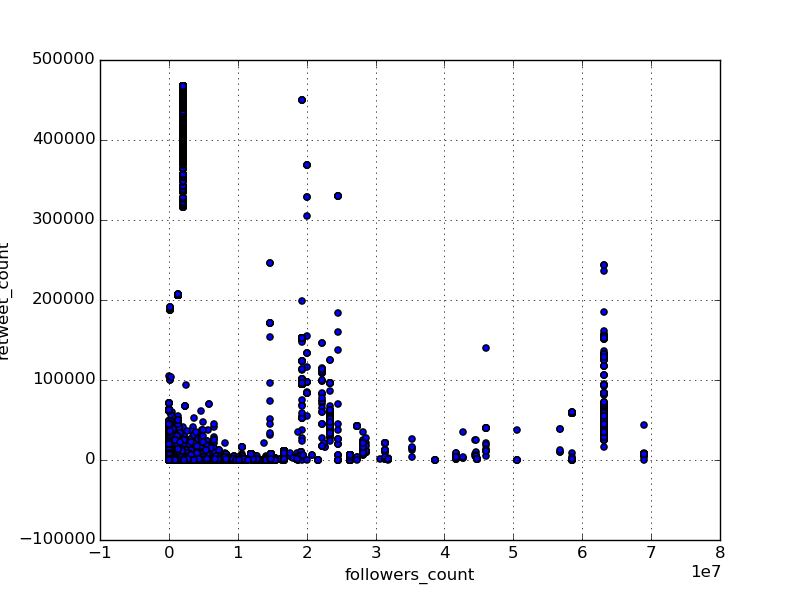
\includegraphics[width=\linewidth]{img/followers_count.png}
    \caption{Followers}
\endminipage\hfill
\minipage[t]{0.25\textwidth}
    \centering
    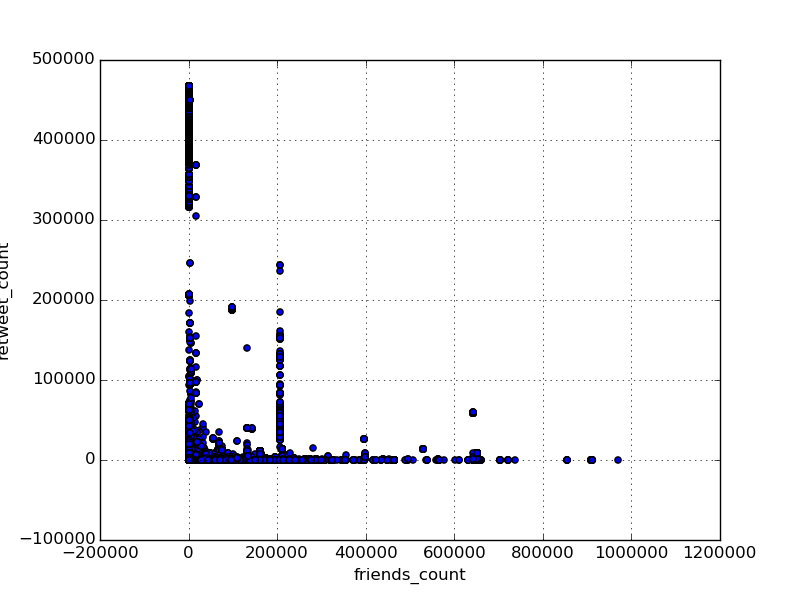
\includegraphics[width=\linewidth]{img/friends_count.png}
    \caption{Friends}
\endminipage\hfill
\minipage[t]{0.25\textwidth}
    \centering
    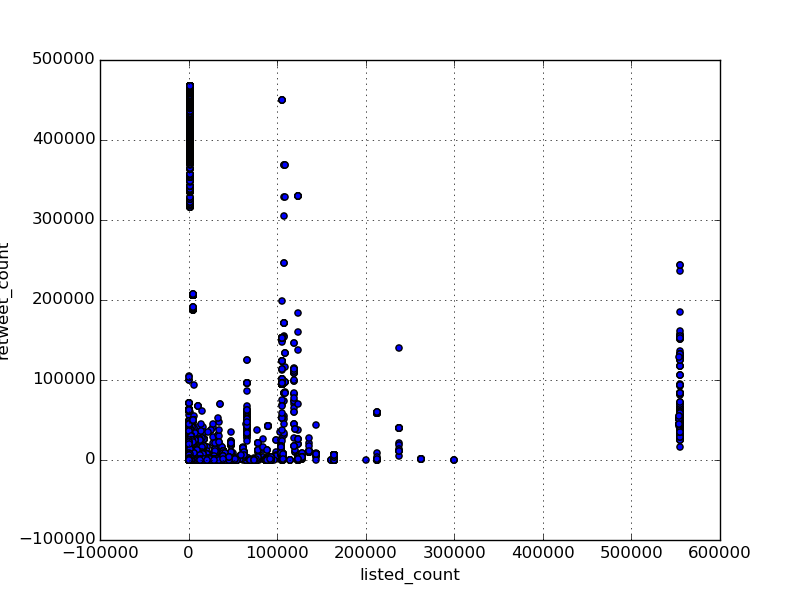
\includegraphics[width=\linewidth]{img/listed_count.png}
    \caption{Listed}
\endminipage\hfill
\minipage[t]{0.25\textwidth}
    \centering
    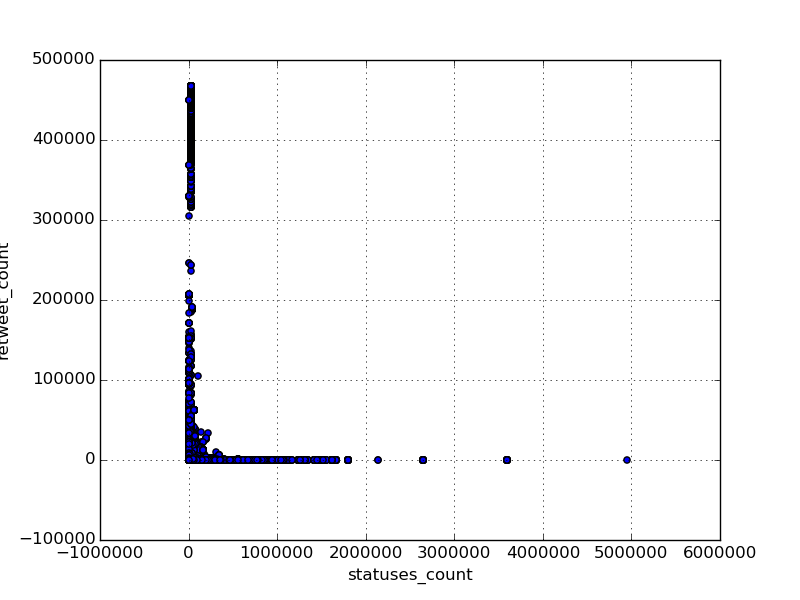
\includegraphics[width=\linewidth]{img/statuses_count.png}
    \caption{Statuses}
\endminipage\hfill
\end{figure}

\begin{figure}[H]
\minipage[t]{0.25\textwidth}
    \centering
    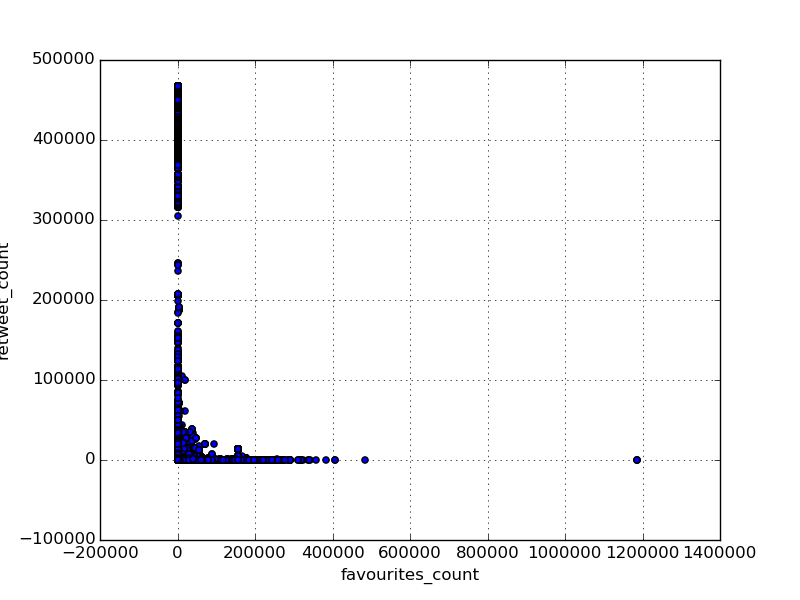
\includegraphics[width=\linewidth]{img/favourites_count.png}
    \caption{Favourites}
\endminipage\hfill
\minipage[t]{0.25\textwidth}
    \centering
    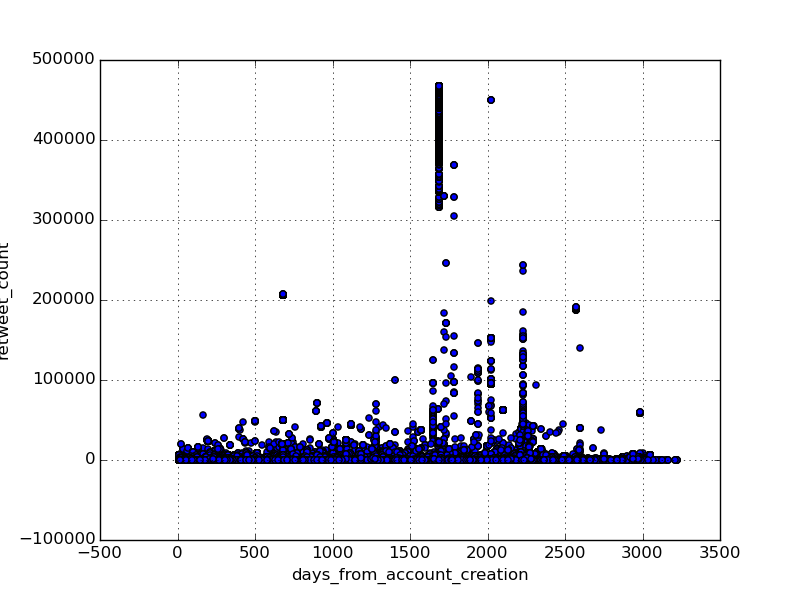
\includegraphics[width=\linewidth]{img/days_from_account_creation.png}
    \caption{Days from account creation}
\endminipage\hfill
\minipage[t]{0.25\textwidth}
    \centering
    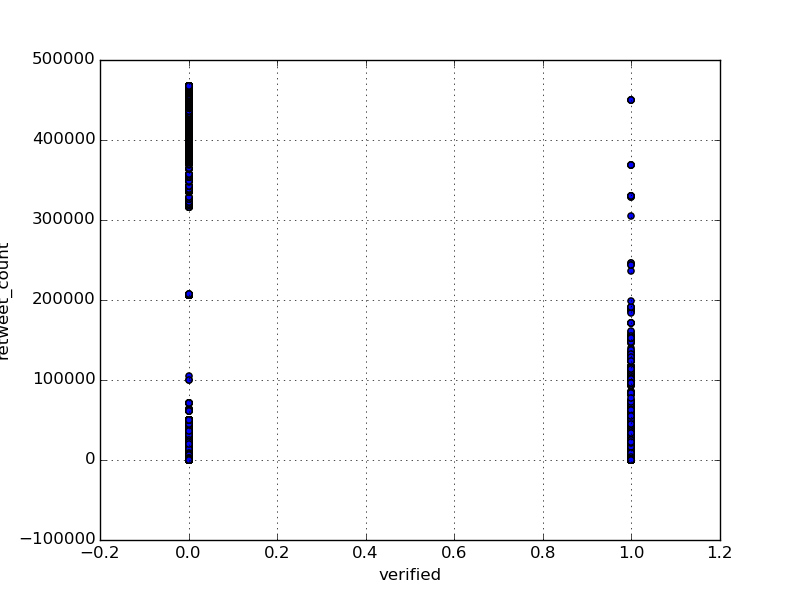
\includegraphics[width=\linewidth]{img/verified.png}
    \caption{Verified boolean}
\endminipage\hfill
\minipage[t]{0.25\textwidth}
    \centering
    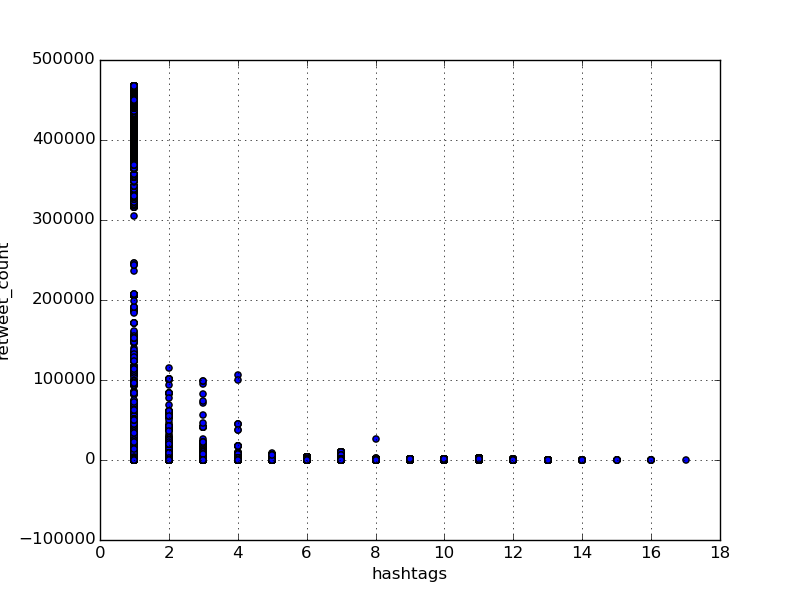
\includegraphics[width=\linewidth]{img/hashtags.png}
    \caption{Hashtags}
\endminipage\hfill
\end{figure}

\begin{figure}[H]
\minipage[t]{0.25\textwidth}
    \centering
    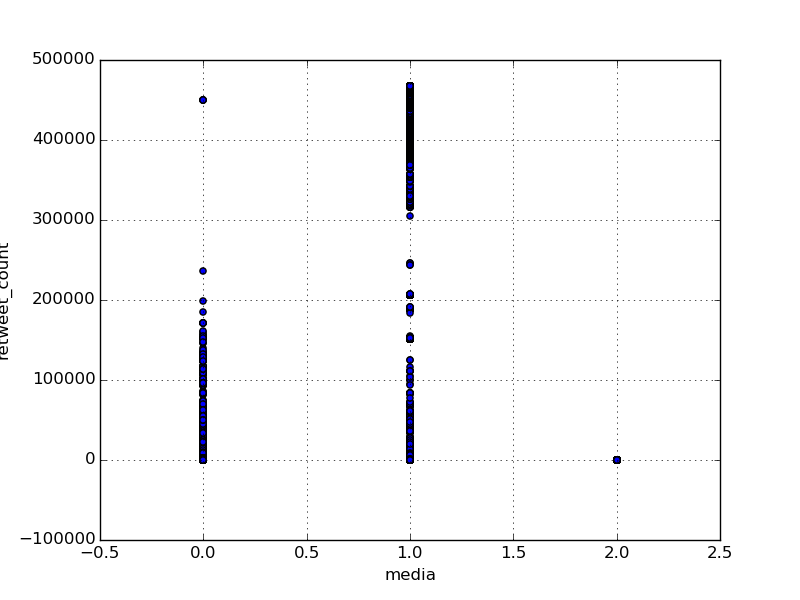
\includegraphics[width=\linewidth]{img/media.png}
    \caption{Media}
\endminipage\hfill
\minipage[t]{0.25\textwidth}
    \centering
    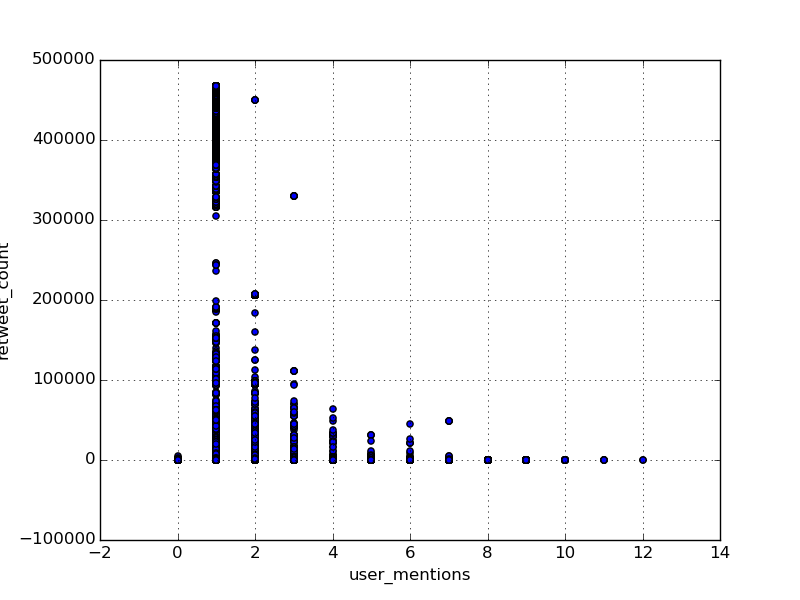
\includegraphics[width=\linewidth]{img/user_mentions.png}
    \caption{User mentions}
\endminipage\hfill
\minipage[t]{0.25\textwidth}
    \centering
    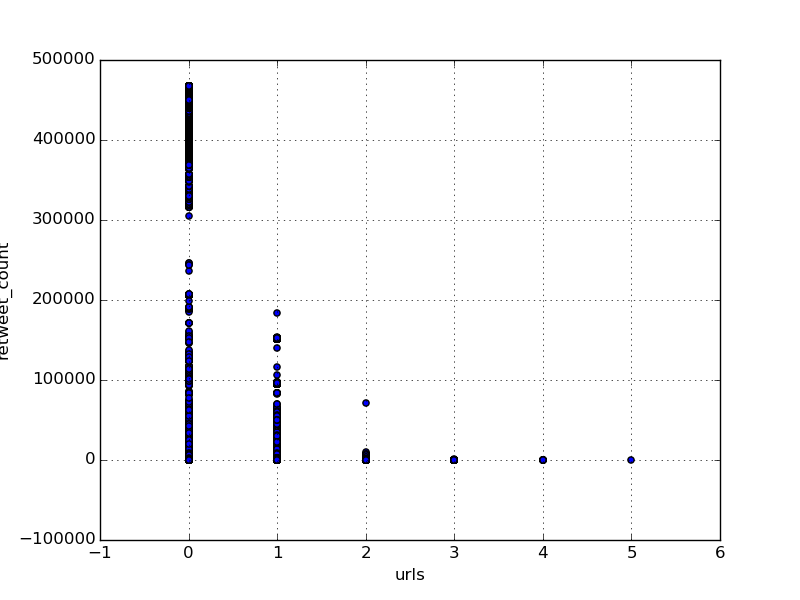
\includegraphics[width=\linewidth]{img/urls.png}
    \caption{URLs}
\endminipage\hfill
\minipage[t]{0.25\textwidth}
    \centering
    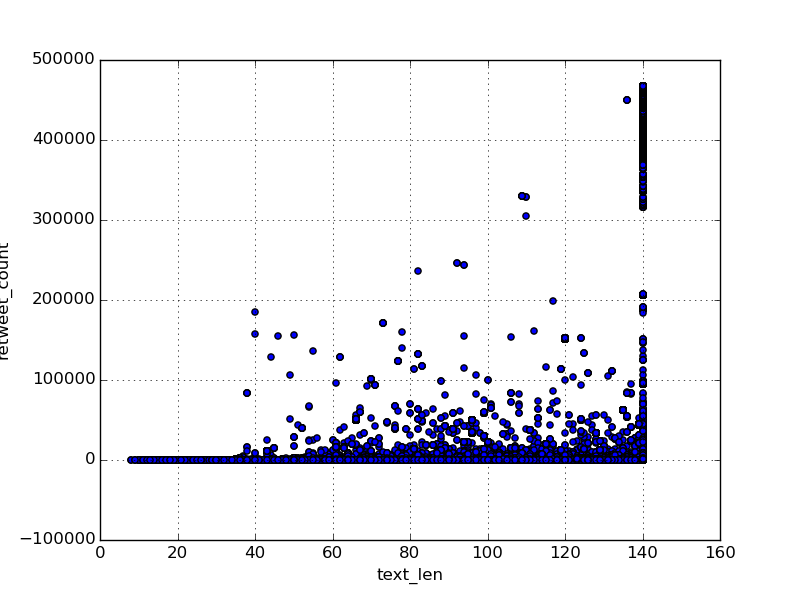
\includegraphics[width=\linewidth]{img/text_len.png}
    \caption{Tweet length}
\endminipage\hfill
\end{figure}

Table \ref{tab:corel} shows the mean, standard deviation and Pearson's correlation coefficients between each feature and the number of retweets.

\begin{table}[h]
\centering
\begin{tabular}{ l | c  | c |c }
\textbf{Feature} & \textbf{Mean}  & \textbf{Std} & \textbf{Correlation} \\\hline
Followers & 576220.62 & 4365041.66 & 0.194274  \\
Friends & 8327.40 & 35412.00 &  0.033895  \\
Listed & 3514.62 &  34121.9 & 0.159713  \\
Statuses  & 43056.14 & 97635.02 & -0.016041  \\
Favourites & 3800.77 & 11700.45 & -0.021614  \\
Account age &  1156.66 & 777.73 & 0.069277  \\
Verified &  0.11 & 0.31 & 0.077538  \\
Hashtags & 1.80 & 1.37 & -0.052247  \\
Media & 0.30 & 0.46 & 0.071278  \\
User mentions &  0.95 & 1.00 & 0.028637  \\
URLs &  0.45 & 0.54 & -0.034712  \\
Tweet length & 113.53 & 28.27 & 0.060207 
\end{tabular}
\caption{Mean, standard deviation and correlations between each feature and the retweet count.}
\label{tab:corel}
\end{table}


\subsection{Model training}
After loading the features and retweet count from the HDFS file, our dataset is balanced in order to increase the weight of viral tweets. This process adds multiple occurrences of every viral tweet in order to create a dataset where the number of popular and non popular tweets is the same. We experimented with different threshold values and got the best results with threshold equal to 55000. Less than 1\% of our tweets reach this threshold. If this process was skipped, the model would essentially focus on non viral tweets, which would give non viral predictions for most of the viral tweets during the testing phase. The balanced dataset is eventually shuffled and divided into two parts. The first 80\% are used as the training set while the last 20\% are used as the testing set.

When considering the model to use, we tried to look at the problem from two perspectives, as a regression and a classification problem. 

\subsubsection{Linear Regression}
The first approach is a linear regression model. The idea of this model is to treat the number of retweets as the dependent variable and all the other features as independent variables. By regression we try to optimize the weights in such a way that the root mean squared error between the actual values and the predicted values is minimized. The algorithm used is a generalized linear model (GLM) called Bayesian Ridge. 

Equation \ref{eq:glm} gives a basic representation of a GLM. $w_0$ represents the intercept term, $w_1$  to  $w_n$ are the values of the coefficients, and $y \in {0,+\infty}$ 

\begin{equation}
\hat{y}(w,x) = w_0 + w_1 x_1 + w_2 x_2 + ... + w_n x_n
\label{eq:glm}
\end{equation}

The weights of the coefficients in figure \ref{fig:coefficients} illustrate the relative importance of the features. A significant positive or negative value indicates that this feature is an important factor to calculate the retweet count. It can be seen that many features have very low regression coefficients. 


\begin{figure}[H]
\centering
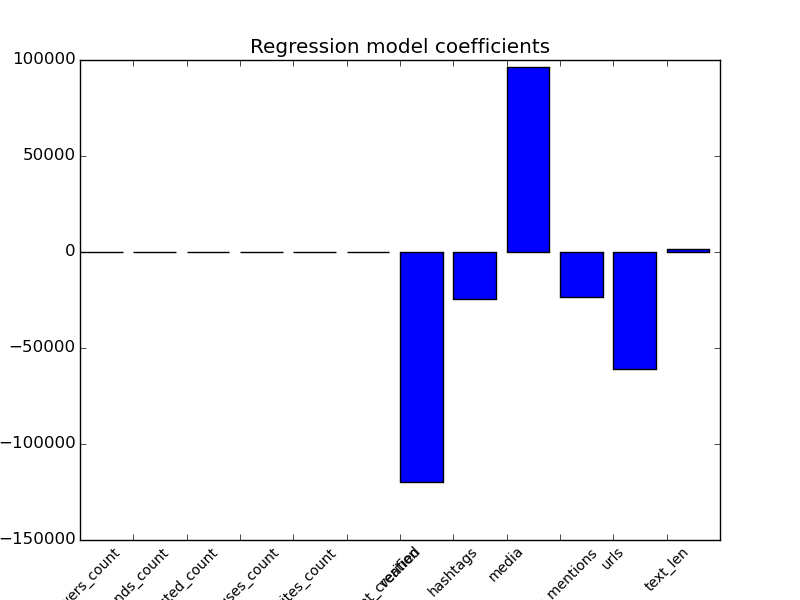
\includegraphics[width=0.6\linewidth]{img/coefficients.png}
% 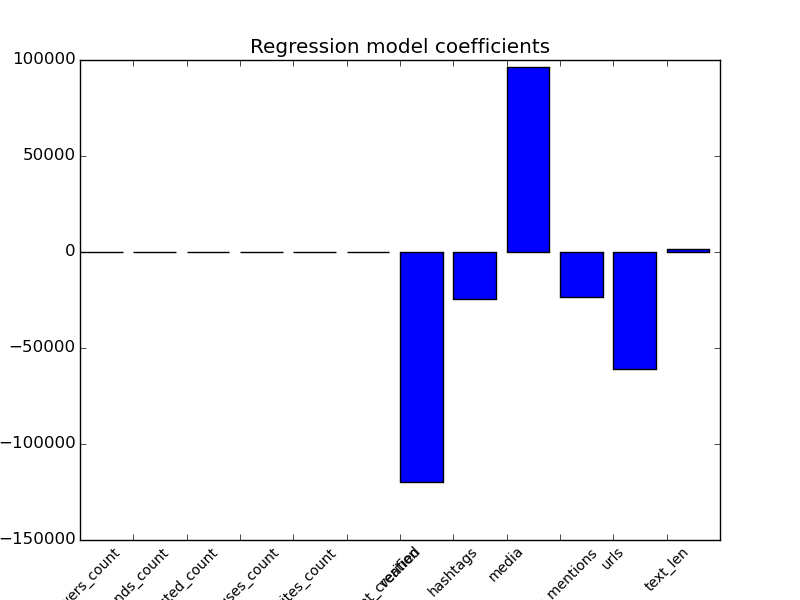
\includegraphics[width=0.6\linewidth]{img/coefficients.png}
\caption{Linear regression coefficients}
\label{fig:coefficients}
\end{figure}


\subsubsection{Classification}
The second approach is to treat the problem as a classification problem. Here, the dependent variable Y is the not number of the retweets, but a class label. The classes are viral and non-viral indicated by 1 or 0, where the boundary between those classes is defined by a threshold applied to the retweet count. This approach should maek the model less sensitive to noise or some spurious viral retweets.

For classification, logistic regression was chosen. Equation \ref{eq:LR} gives a basic representation of a logistic regression. 

\begin{equation}
\hat{y}(w,x) = [exp (w_0 + w_1 x_1 + ... + w_n x_n)] / [1 + exp (w_0 + w_1 x_1 + ... + w_n x_n)]
\label{eq:LR}
\end{equation}

Logistic regression is a method for fitting a regression curve, \textbf{y} = \textbf{f(x)}, when y consists of proportions, or binary coded (0,1--failure,success) data. When the response is a binary variable, and x is numerical, logistic regression fits a logistic curve given above to the relationship between x and y.

When looking at the coefficients of each feature in Figure \ref{fig:coefficientsLR}, we observe that the number of followers improves the probability of a tweet being retweeted significantly, which is also observed as celebrity accounts tend to have a very high number of followers. We also see the presence of media in a tweet, account age and length of a tweet also have a positive impact. On the other hand, features like friends count, favourites count and hashtags have a negative impact. This could also be due to confounding effects from other features, but we could not fully explore it.



\begin{figure}[H]
\centering
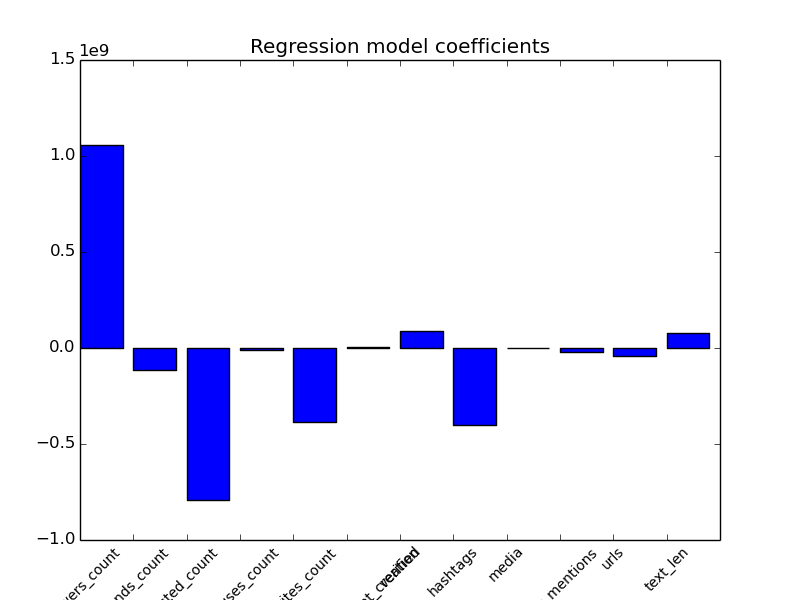
\includegraphics[width=0.6\linewidth]{img/coefficientsLR1.png}
% 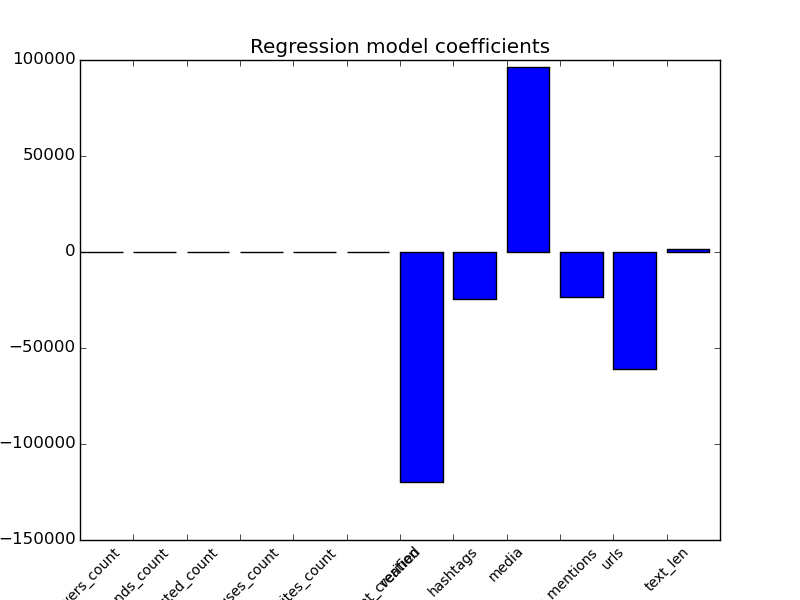
\includegraphics[width=0.6\linewidth]{img/coefficients.png}
\caption{Logistic regression coefficients}
\label{fig:coefficientsLR}
\end{figure}


\subsection{Virality prediction}
In a next step, we used the trained model to predict the virality of hashtags. To be able to discover potentially viral hashtags, we iterate over all hashtags in the inverted index and predict the virality of the tweets containing that hashtag. The virality of the hashtags is then simply computed by taking the sum of the virality of the tweets containing that hashtag. In a final step, the hashtags are sorted in decreasing order by their predicted virality. This approach enables the creation of a top-K list of viral hashtags. 

Additionally, we implemented a search functionality which allows a user to search for a hashtag of interest. Tweets containing the given hashtags that were posted during a specified time frame are then retrieved and their features are extracted. Afterwards the virality of each tweet is predicted. If the predicted virality for that hashtag exceeds a certain threshold, the hashtag is then assumed to be viral. 

\section{Results}
We now want to measure the performances of our model on the testing dataset.

\subsection{Regression}
The first part of figure \ref{fig:results} illustrates the predicted retweet count (Y-axis) according to the expected retweet count, the second part shows the difference between the prediction and expectation. 


\begin{figure}[H]
\centering
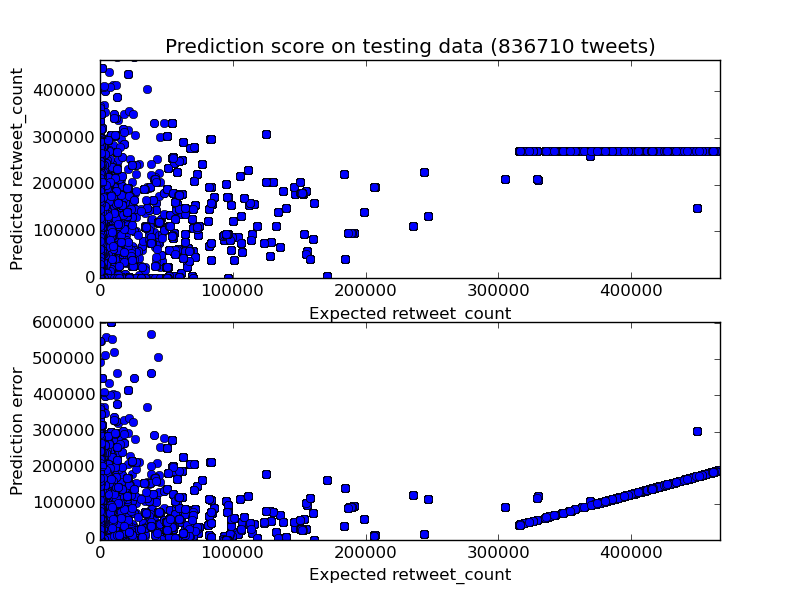
\includegraphics[width=0.6\linewidth]{img/prediction_error.png}
\caption{Linear regression predictions on testing dataset}
\label{fig:results}
\end{figure}

We can observe that the prediction error for viral tweets is quite low. However, lots of false positive are generated by our model, i.e. high retweet counts are predicted when the actual retweet count is low. The most likely explanation for this is that the relationship between some of the features and the retweet count simply are not linear. This is supported by the correlation plots in Section \ref{sec:analyis}.


\subsection{Classification}

On a balanced data set, the logistic regression model was able to correctly predict the virality score on the test set with an accuracy of more than $90\%$.

Figure \ref{fig:resultsLR} visualizes the number of true positives $tp$ (classifier correctly predicts virality), true negatives $tn$ (classifier correctly predicts non-virality), false positives $fp$ (classifier incorrectly predicts virality) as well as false negatives $fn$ (classifier incorrectly predicts non-virality) for a threshold of 50'000. It can be seen that the classifier correctly predicts both virality scores of 1 and 0 with a similar rate (true positives and true negatives). The error rate of false positives and false negatives is also similar. 

We also present the performance of the classifier for different values of thresholds. Table \ref{tab:roc} shows a jump in the true positive rate when we change the threshold value to 55'000. Afterwards, the true positive rate saturates and we notice a reduction in the false positive rate. However, this reduction is not very steep. This indicates that for our data set, the modelling function becomes much more discriminative at a threshold of 55'000. 


\begin{table}[h]
\centering
\begin{tabular}{ l | c |c |}
\textbf{Threshold} & \textbf{True Positive Rate} &
\textbf{False Positive Rate}  \\\hline
25'000  &  89.05  & 6.71  \\
50'000  &  90.94  & 10.00  \\
55'000  &  98.6   & 5.60  \\ 
75'000  &  98.33  & 5.93  \\ 
90'000  &  98.21  & 4.25
\end{tabular}
\caption{ROC Performace of the classifier}
\label{tab:roc}
\end{table}


\begin{figure}[H]
\centering
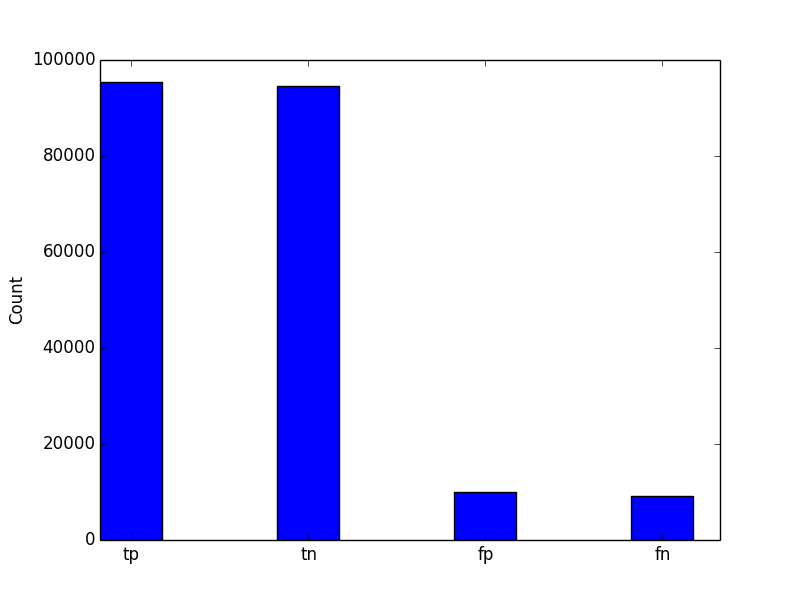
\includegraphics[width=0.6\linewidth]{img/performanceLR.png}
\caption{Logistic regression predictions on testing dataset}
\label{fig:resultsLR}
\end{figure}

\subsection{Virality prediction}
\label{sec:viral}
Table \ref{tab:results} shows the top-10 predicted viral hashtags for the first May week 2015. It can be observed that the hashtags relate to some of the most-covered events at the time. For example, the Baltimore riots, the earthquake in Nepal or the planned execution of Mary Jane Veloso. While the regression and classification predictions share the same top-4 results, the other results do not overlap with the exception of the hashtag ``NepalEarthquake''. 


\begin{table}[h]
\centering
\begin{tabular}{ l | c |c |c}
\textbf{Rank} & \textbf{Regression} &
\textbf{Classification}  \\\hline
1  &  BaltimoreRiots  &  BaltimoreRiots \\
2  &  BestFandomCA2015  &  BestFandomCA2015 \\
3  &  FreddieGray  &  FreddieGray \\
4  &  Baltimore  &  Baltimore \\
5  &  NepalEarthquake  & MGWV \\
6  &  SOL2015  & NepalEarthquake  \\
7  &  LIAMISTHEPOOLCLEANER  &  FOLLOW \\
8  &  HappyKyuziziDay  &  RT \\
9  &  HowIBecameAFan  &  FOLLOWTRICK \\
10  & SaveMaryJaneVeloso   &  Nepal
\end{tabular}
\caption{Top-10 predicted viral hashtags for the first May week 2015}
\label{tab:results}
\end{table}


\section{Discussion}

Our results show that there is some promise in the approach of a feature-based virality prediction. In particular the classification approach seems worth pursuing further. 

One limitation of the current implementation that becomes clear when looking at the top-10 virality predctions in Section \ref{sec:viral} is that it favors hashtags which are already popular at the time of data acquisition as popular hashtags at the time will be more often featured in the inverted index and therefore more tweets will be taken into account for already popular hashtags. However, predicting the virality of hashtags which are not popular already is a difficult problem. The regression model does allow the prediction of high virality for non popular hashtags if the contained tweets have high retweet count predictions, for example if the tweets are created by very influential authors. However, this is not case in the classification model as it only distinguishes between two classes, viral and non-viral. 

Therefore, one extension to the classification approach would be to classify the virality of a tweet into more than two classes. For example, the virality could be divided into different classes of a certain number of retweets. This would potentially allow for a more precise and fine-grained virality prediction when using the classification approach. 

Another area that needs more development and fine-tuning lies in the chosen approach to the problem of predicting virality and our choice of features. 
One area which could be further explored is sentiment analysis of tweets. Due to the restricted length of a tweet, traditional approaches to sentiment analysis are not perfectly suited for Twitter data. Dedicating more time into researching and implementing a suitable sentiment analysis for Twitter data could therefore be a promising direction to take. 
Another aspect that is currently not taken into account is the community structure of Twitter, which could also serve as an improvement to the project. 




\section{Conclusion}

The work done in this project shows the feasibility of predicting the virality of tweets using a feature-based approach. While past research has focused on the virality prediction of individual tweets, this work integrates these ideas with concepts from information retrieval to create a novel approach to predicting the virality of hashtags. The results of our work show some promise but further research into other fields such as social media analysis will be needed to obtain more accurate and reliable results.


% Removed to fit report on 10 pages
%    \pagebreak
    
    \bibliographystyle{plain}
    \renewcommand{\bibname}{References}
    \bibliography{references}


    %\backmatter
\end{document}